\RequirePackage{fix-cm}
\documentclass[a4paper,ngerman]{scrartcl}

\usepackage[utf8]{inputenc}
\usepackage{cmbright}
\usepackage[T1]{fontenc}
\usepackage{babel}
\DeclareUnicodeCharacter{FEFF}{}

\usepackage{paralist}	
\usepackage{geometry}	
\usepackage{tabularx}		
\usepackage{listings} 
\usepackage{datetime} 
\usepackage{graphicx}
\usepackage{enumitem}
\usepackage{booktabs}
\usepackage{multirow}
\usepackage{newunicodechar} 

\usepackage{color}
\usepackage{varioref} 
\usepackage[colorlinks=false, pdfborder={0 0 0}]{hyperref} 
\usepackage{cleveref} 

\setcounter{secnumdepth}{2} 
  
\definecolor{bluekeywords}{rgb}{0,0,1}
\definecolor{greencomments}{rgb}{0,0.5,0}
\definecolor{redstrings}{rgb}{0.64,0.08,0.08}
\definecolor{xmlcomments}{rgb}{0.5,0.5,0.5}
\definecolor{types}{rgb}{0.17,0.57,0.68}

\usepackage{listings}
\lstset{language=[Sharp]C,
	captionpos=b,
	showspaces=false,
	showtabs=false,
	breaklines=true,
	showstringspaces=false,
	breakatwhitespace=true,
	escapeinside={(*@}{@*)},
	commentstyle=\color{greencomments},
	morekeywords={partial, var, value, get, set, namespace},
	keywordstyle=\color{bluekeywords},
	stringstyle=\color{redstrings},
	basicstyle=\ttfamily\small,
	extendedchars=\true,
}

\begin{document}
\title{AmazingGeoRace}
\subtitle{MOC5-Projekt}
\author{Stefan Kert}
\date{\today}
\maketitle
\section{Allgemeines}
Die Plattform, welche für die Projektarbeit ausgewählt wurde, ist Windows Phone 8.1. Es gibt bei der Version 8.1 der Plattform zahlreiche Vorteile, wie zum Beispiel eine bessere Unterstützung des .Net Frameworks und im Allgemeinen ist es zukunftsorientierter gestaltet. Als IDE wurde Visual Studio 2015 in der Enterprise Version verwendet und getestet wurde die App auf einem Emulator mit WP 8.1 und einem Emulator mit WP 10. 

\subsection{Tombstoning in WP 8.1}
Bei der Architektur von WP 8.1 hat sich Microsoft für einen ähnlichen Weg für das Lifecycle Management entschieden wie beim WP 8. Einer der größten Unterschiede ist die Tatsache, dass Apps nicht mehr direkt beendet oder deaktiviert werden, sondern in den sogenannten \textit{Suspended}-Status versetzt werden. Bei Speicherknappheit, kann es vorkommen, dass die App denoch komplett beendet wird. Dies geschieht wie auch beim WP 8 ohne Vorwarnung und daher sollte sichergestellt werden, dass bei jedem Übergang in den \textit{Suspended}-Status alle benötigten Daten gespeichert werden. Für diese Zwecke können in WP 8.1 die in der Klasse Application vorhandenen Methoden \textit{OnLaunched} überschrieben, bzw. \textit{OnSupsended} auf das \textit{Suspended} Event gebunden werden. Dort wird ähnlich wie beim WP 8 auf ein \textit{SessionState}-Dictionary zugegriffen, welches schließlich im System persistiert wird. Sobald das \textit{OnLaunched} Event aufgerufen wird, können die Daten aus diesem Dictionary erneut geladen werden. Weiters gibt es die Möglichkeit zum Speichern der aktuell geöffneten Frame, sodass diese beim erneuten Öffnen wieder geöffnet wird. 

\section{Lösungsidee}
Bei der Lösung wird auf eine möglichst gute Trennung der einzelnen Aspkete geachtet. Es wird dabei das in der .NET Programmierungsumgebung etablierte MVVM Pattern  verwendet. Durch dieses wird eine gute Trennung zwischen View und Logik gewährleistet. Weiters wird eine eigene Klasse für die Interaktion mit dem Webservice implementiert. 


\subsection{Anwendungsarchitektur}
Grundsätzlich besteht die AmazingGeoRace-App aus 3 Seiten und mehreren Dialogen:
\begin{itemize}
	\item LoginPage - Hier wird dem User die Möglichkeit gegeben sich anzumelden. Dabei wird bei falschen Logindaten eine Fehlermeldung ausgegeben und bei erfolgreicher Anmeldung weitergeleitet. Nachdem erfolgreicher Anmeldung werden die Logindaten bei jedem Beenden der App persistiert und der Benutzer kann so eingeloggt bleiben. 
	\item MainPage: Hier werden alle für den Benutzer vorhandenen Routen aufgelistet und der Benutzer kann sich eine Route aussuchen. Es wird dem Benutzer außerdem mitgeteilt, ob eine Route bereits erfolgreich abgeschlossen wurde. Dies erfolgt durch einen grünen Haken neben dem Namen der Route. Weiters gibt es die Möglichkeit alle Routen zurückzusetzen und sich auszuloggen. 
	\item RaceDetailsPage: Nach der Auswahl einer Route wird auf diese Seite weitergeleitet. Auf dieser Seite hat der Benutzer die Möglichkeit die einzelnen Checkpoints auf einer Karte zu sehen. Weiters wird dem Benutzer der Name, sowie ein Hinweis für den aktuellen Checkpoint angezeigt. Wenn der Benutzer eine Lösung angeben möchte gibt es dafür einen Button. Durch ein tippen auf diesen Button kommt der Benutzer zum SolutionDialog wo er die Lösung angeben kann. Bei erfolgreicher Eingabe im SolutionDialog bekommt der Benutzer eine Erfolgsmeldung und der nächste Checkpoint wird angezeigt. Es werden außerdem für alle bereits passierten Checkpoints Punkte bzw. Linien zwischen den einzelnen Checkpoints auf der Karte eingezeichnet. Bei falscher Eingabe wird der Benutzer darüber informiert, dass die angegebene Lösung falsch war. Wenn der Benutzer den letzten Checkpoint erfolgreich freigeschalten hat bekommt er eine Erfolgsmeldung und das Interface der RaceDetailsPage ändert sich, sodass jetzt nur noch die Karte und ein Button zum Zurücksetzen der aktuellen Route vorhanden sind. Bei Tippen auf diesen Button wird die aktuelle Route zurückgesetzt und die Seite neu geladen und die Schnitzeljagd kann von neuem beginnen.
\end{itemize}

\subsection{Implementierungsdetails}
\subsubsection{Architektur}
Wie bereits erwähnt ist die Anwendung mit dem für .NET Applikationen üblichen MVVM Pattern umgesetzt, wo die View über das ViewModel bescheid weiß, das ViewModel aber keine Referenz auf dei View besitzt. Das ViewModel wiederum weiß bescheid, wie es die Daten auslesen kann. Dies wird über den ServiceProxy erledigt, welcher wiederum auf den Webservice zugreift, welcher den Zugriff auf den Webservice kapselt. Ein weiterer wichtiger Bestandteil ist die Klasse Loginservice, welche weiderum vom ServiceProxy abhängt und die Funktionalität zum Authentifizieren und zum Speichern der Logindaten bietet. Die beschrieben Architektur ist in Abb. \ref{fig:arch} dargestellt. 

\begin{figure}[h]
\centering
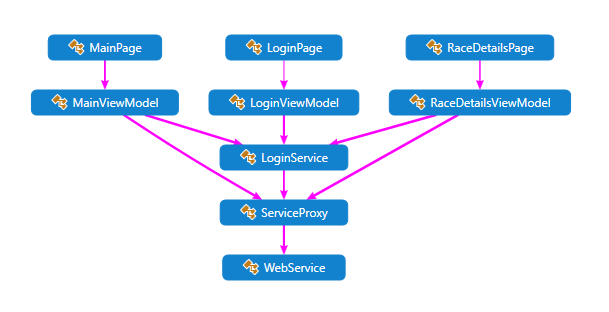
\includegraphics[width=.80\textwidth]{images/architecture}
\caption{Architektur}
\label{fig:arch}
\end{figure}

\newpage
\section{Testfälle und Screenshots}
In diesem Abschnitt werden Screenshots für die einzelnen Testfälle gezeigt. Diese sind dabei nach Seiten gruppiert.

\subsection{LoginPage}
Für die Loginpage gibt es nur zwei Testfälle. Einerseits, dass der Login erfolgreich war, dann wird die MainPage angezeigt. Andererseits, dass der Login nicht erfolgreich war, dann wird das in Abb. \ref{fig:ScreenLogin} rechts dargestellte Fenster angezeigt. Der Basisdialog zur Eingabe befindet sich in Abb. \ref{fig:ScreenLogin} links.

\begin{figure}[h]
	\centering
	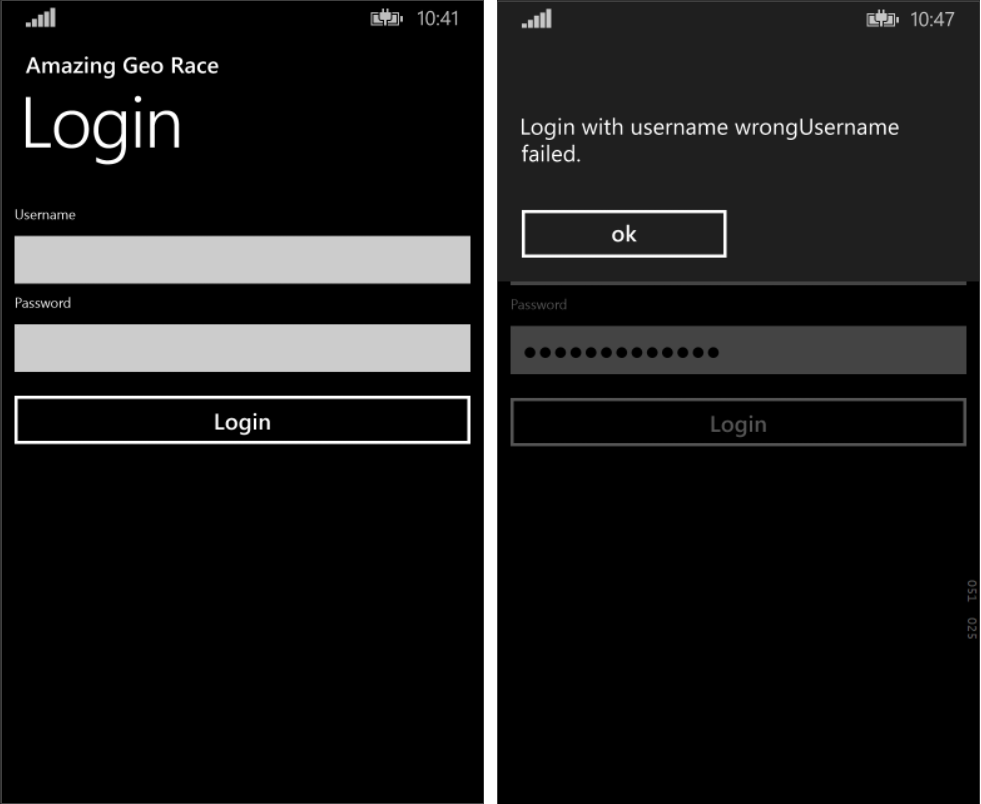
\includegraphics[width=.95\textwidth]{images/loginPage_Stati}
	\caption{Login}
	\label{fig:ScreenLogin}
\end{figure}

\newpage
\subsection{MainPage}
Beim erstmaligen Öffnen der Mainpage sollte das in  Abb. \ref{fig:ScreenMain} ganz links dargestellte Bild angezegit werden. Es sind noch keine Routen abgeschlossen und daher wird dem Benutzer auch kein Erfolgszeichen angezeigt. Das mittlere Bild stellt den Fall dar, dass der Benutzer bereits eine Route abgeschlossen hat, es wird ein grünes Häckchen angezeigt. Beim ganz rechten Bild handelt es sich um den Fall, dass der Benutzer die Routen zurückgesetzt hat. Bei Erfolg wird er darüber informiert, dass alle Routen zurückgesetzt sind. Beim Klicken des Logout Buttons wird der Benutzer zum Homescreen des WP weitergeleitet.
\begin{figure}[h]
	\centering
	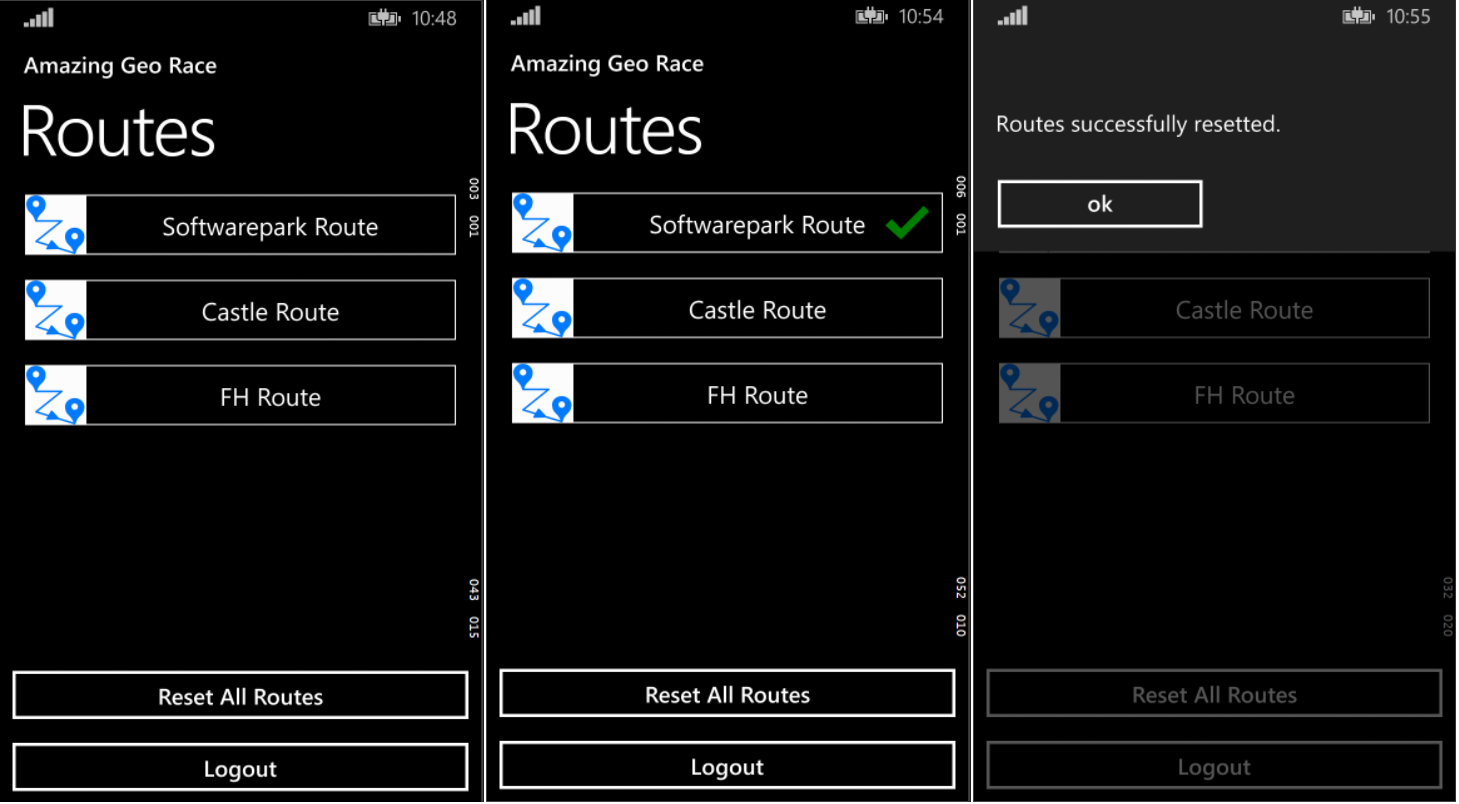
\includegraphics[width=.95\textwidth]{images/routePage_Stati}
	\caption{MainPage}
	\label{fig:ScreenMain}
\end{figure}

\newpage
\subsection{RaceDetailsPage}
Nachdem Auswählen einer Route auf der Mainpage wird dem Benutzer das in Abb. \ref{fig:ScreenDetails} ganz links angezeigte Fenster angezeigt, falls der Benutzer diese Route noch nicht erfolgreich abgeschlossen hat. Wenn alle Checkpoints freigeschalten wurden und das Ziel erreicht wurde, oder falls er eine bereits abgeschlossene Route noch einmal öffnet, wird dem Benutzer die in der Mitte der Abb. \ref{fig:ScreenDetails} gezeigte Seite angezeigt. Auf dieser Seite kann der Benutzer wiederum die aktuelle Route zurücksetzen. Bei Erfolg wird dem Benutzer die ganz rechts dargestellte Seite angezeigt. Wenn der Benutzer auf den \textit{ProvideSolution} Button klickt, wird ihm der SolutionDialog angezeigt.
\begin{figure}[h]
	\centering
	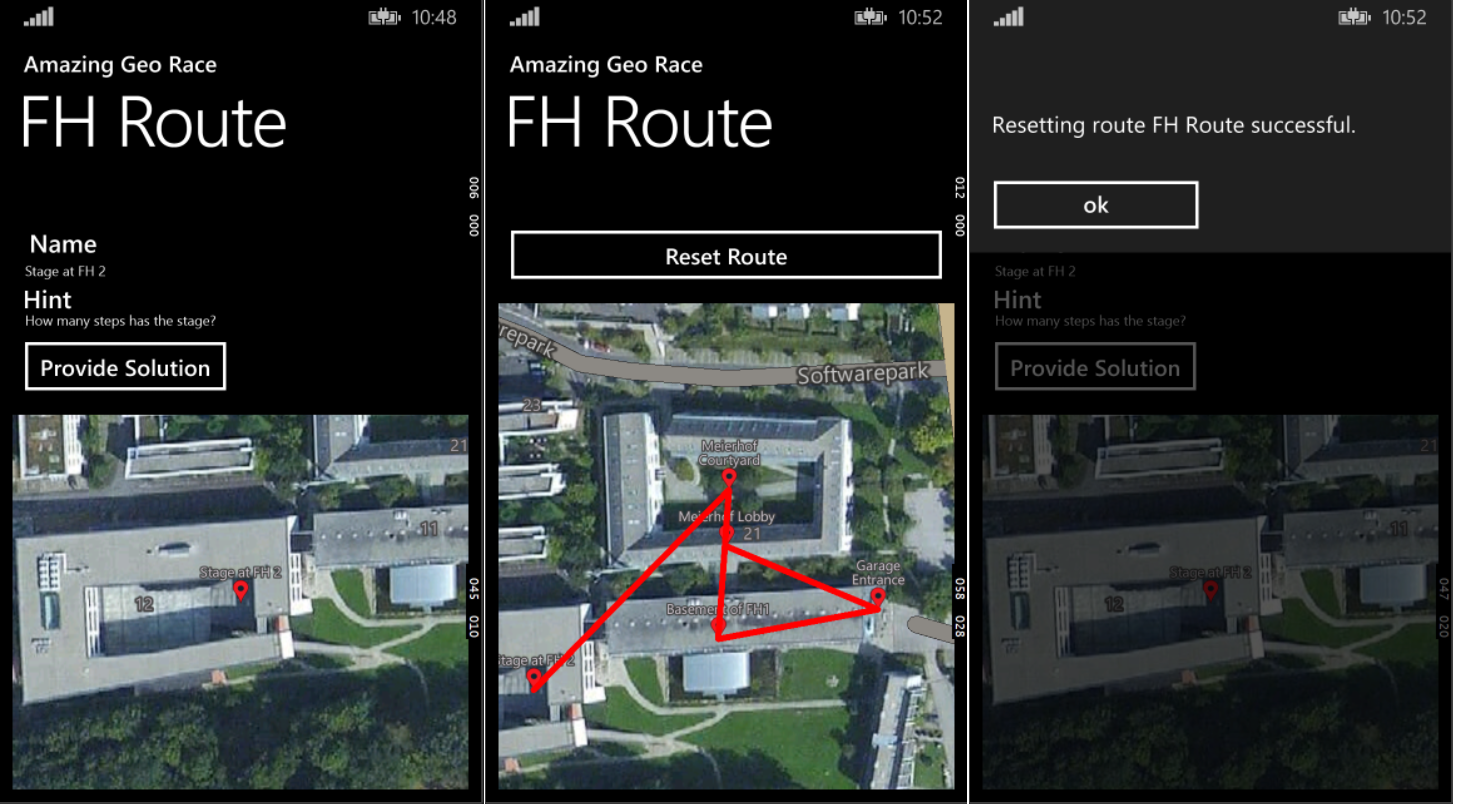
\includegraphics[width=.95\textwidth]{images/routeDetailsPage_Stati}
	\caption{RaceDetailsPage}
		\label{fig:ScreenDetails}
\end{figure}


\newpage
\subsection{SolutionDialog}
Beim Öffnen des SolutionDialogs wird dem Benutzer ein Overlay mit leerem Textfeld und zwei Buttons angezeigt, wo die Lösung eingegeben werden kann. Bei Erfolg wird dem Benutzer die Meldung \textit{Congratulations. Correct answer!} ausgegeben. Bei einer falschen Lösung wird der Benutzer mit einer Fehlermeldung darüber informiert, dass diese Lösung falsch war. Sobald der Benutzer die Lösung für den letzten Checkpoint richtig angegeben hat, wird er darüber informiert, dass die Route erfolgreich abgeschlossen wurde. Diese Fälle sind in  \ref{fig:ScreenSolution} dargestellt.

\begin{figure}[h]
	\centering
	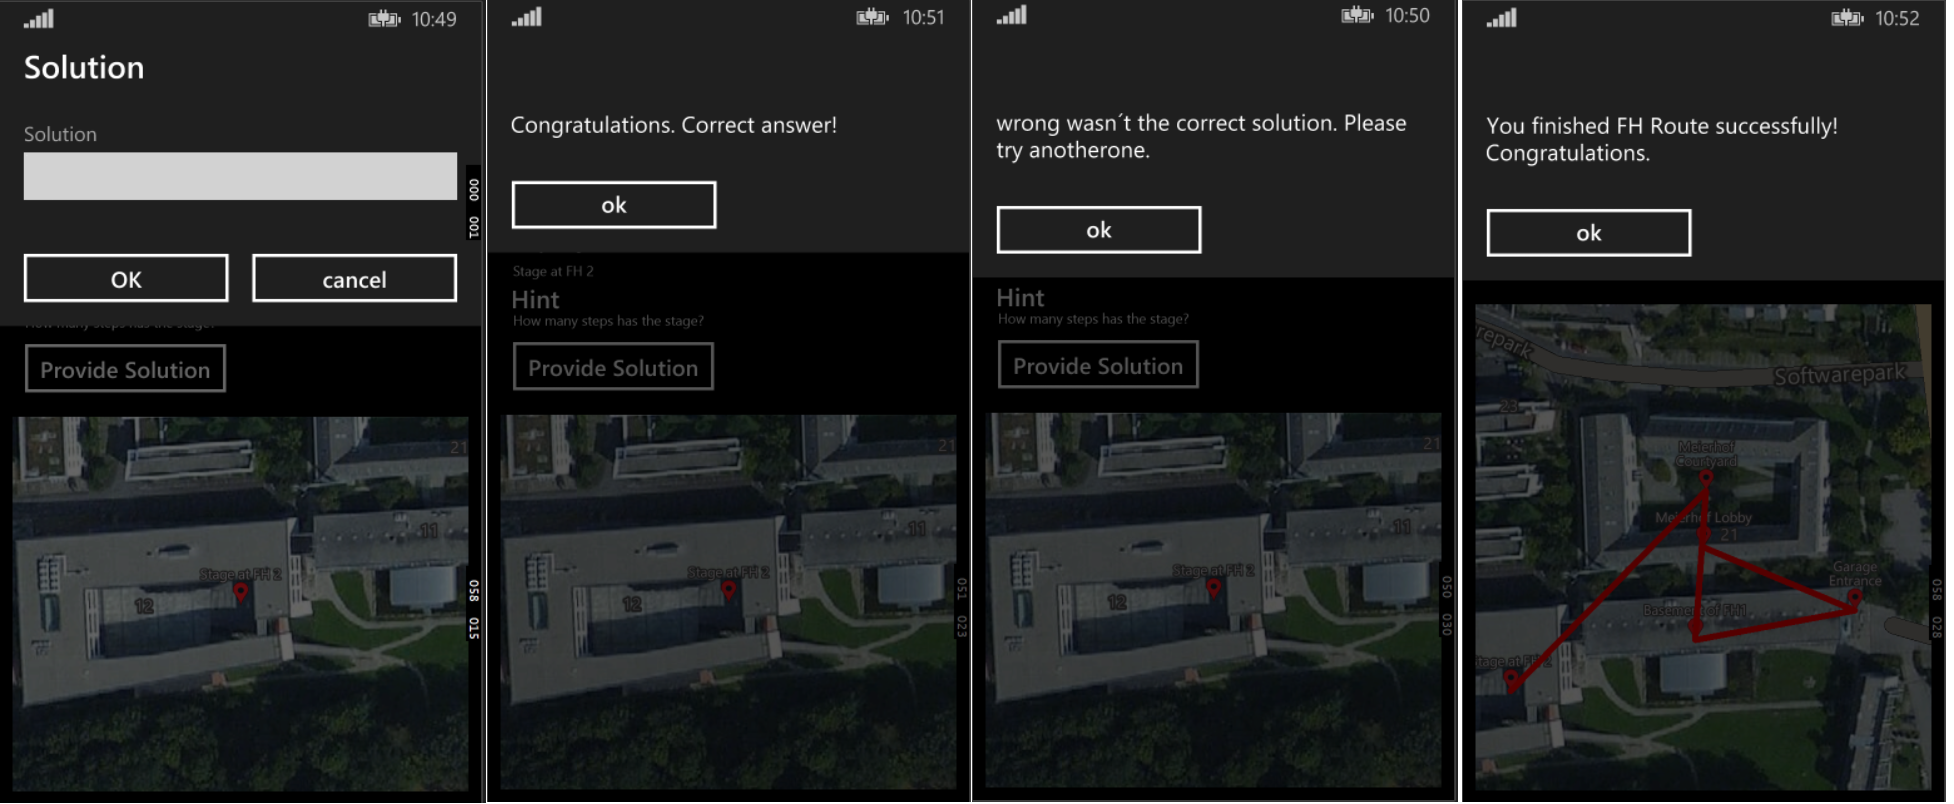
\includegraphics[width=.95\textwidth]{images/routeSolutionPage_Stati}
	\caption{SolutionDialg}
		\label{fig:ScreenSolution}
\end{figure}



\newpage
\section{Quellcode}

\subsection{Commands}
\lstinputlisting[caption=RelayCommand.cs]{../AmazingGeoRace/AmazingGeoRace/Commands/RelayCommand.cs}

\subsection{Common}
\lstinputlisting[caption=ExceptionHandling.cs]{../AmazingGeoRace/AmazingGeoRace/Common/ExceptionHandling.cs}
\lstinputlisting[caption=MessageBoxWrapper.cs]{../AmazingGeoRace/AmazingGeoRace/Common/MessageBoxWrapper.cs}
\lstinputlisting[caption=NavigationHelper.cs]{../AmazingGeoRace/AmazingGeoRace/Common/NavigationHelper.cs}
\lstinputlisting[caption=ObservableDictionary.cs]{../AmazingGeoRace/AmazingGeoRace/Common/ObservableDictionary.cs}
\lstinputlisting[caption=SuspensionManager.cs]{../AmazingGeoRace/AmazingGeoRace/Common/SuspensionManager.cs}

\subsection{Converters}
\lstinputlisting[caption=BooleanToCollapsedConverter.cs]{../AmazingGeoRace/AmazingGeoRace/Converters/BooleanToCollapsedConverter.cs}
\lstinputlisting[caption=BooleanToVisibilityConverter.cs]{../AmazingGeoRace/AmazingGeoRace/Converters/BooleanToVisibilityConverter.cs}

\subsection{Data}
\lstinputlisting[caption=WebService.cs]{../AmazingGeoRace/AmazingGeoRace/Data/WebService.cs}

\subsection{Domain}
\lstinputlisting[caption=LoginService.cs]{../AmazingGeoRace/AmazingGeoRace/Domain/LoginService.cs}
\lstinputlisting[caption=ServiceProxy.cs]{../AmazingGeoRace/AmazingGeoRace/Domain/ServiceProxy.cs}

\subsection{Models}
\lstinputlisting[caption=Checkpoint.cs]{../AmazingGeoRace/AmazingGeoRace/Models/Checkpoint.cs}
\lstinputlisting[caption=CheckpointRequest.cs]{../AmazingGeoRace/AmazingGeoRace/Models/CheckpointRequest.cs}
\lstinputlisting[caption=Request.cs]{../AmazingGeoRace/AmazingGeoRace/Models/Request.cs}
\lstinputlisting[caption=Route.cs]{../AmazingGeoRace/AmazingGeoRace/Models/Route.cs}
\lstinputlisting[caption=RouteRequest.cs]{../AmazingGeoRace/AmazingGeoRace/Models/RouteRequest.cs}

\subsection{ViewModels}
\lstinputlisting[caption=LoginViewModel.cs]{../AmazingGeoRace/AmazingGeoRace/ViewModels/LoginViewModel.cs}
\lstinputlisting[caption=MainViewModel.cs]{../AmazingGeoRace/AmazingGeoRace/ViewModels/MainViewModel.cs}
\lstinputlisting[caption=RaceDetailsViewModel.cs]{../AmazingGeoRace/AmazingGeoRace/ViewModels/RaceDetailsViewModel.cs}
\lstinputlisting[caption=ViewModelBase.cs]{../AmazingGeoRace/AmazingGeoRace/ViewModels/ViewModelBase.cs}

\subsection{Views-Markup}
\lstinputlisting[caption=LoginPage.xaml]{../AmazingGeoRace/AmazingGeoRace/Views/LoginPage.xaml}
\lstinputlisting[caption=MainPage.xaml]{../AmazingGeoRace/AmazingGeoRace/Views/MainPage.xaml}
\lstinputlisting[caption=RaceDetailsPage.xaml]{../AmazingGeoRace/AmazingGeoRace/Views/RaceDetailsPage.xaml}
\lstinputlisting[caption=SolutionDialog.xaml]{../AmazingGeoRace/AmazingGeoRace/Views/SolutionDialog.xaml}

\subsection{Views}
\lstinputlisting[caption=LoginPage.xaml.cs]{../AmazingGeoRace/AmazingGeoRace/Views/LoginPage.xaml.cs}
\lstinputlisting[caption=MainPage.xaml.cs]{../AmazingGeoRace/AmazingGeoRace/Views/MainPage.xaml.cs}
\lstinputlisting[caption=RaceDetailsPage.xaml.cs]{../AmazingGeoRace/AmazingGeoRace/Views/RaceDetailsPage.xaml.cs}
\lstinputlisting[caption=SolutionDialog.xaml.cs]{../AmazingGeoRace/AmazingGeoRace/Views/SolutionDialog.xaml.cs}

\subsection{App}
\lstinputlisting[caption=App.xaml]{../AmazingGeoRace/AmazingGeoRace/App.xaml}
\lstinputlisting[caption=App.xaml.cs]{../AmazingGeoRace/AmazingGeoRace/App.xaml.cs}

\end{document}